\documentclass[../../../interview-questions.tex]{subfiles}

\begin{document}

\subsection{Filter和Interceptor区别}

\paragraph{实现原理不同-实现原理}

Filter是基于函数回调(doFilter()方法)的,而Interceptor则是基于Java反射的(AOP思想)。拦截器的执行是在穿插在SpringMvc的工作流程中的,并没有用到动态代理机制,直接调用的拦截器方法。自定义的过滤器中都会实现一个 doFilter()方法,这个方法有一个FilterChain 参数,而实际上它是一个回调接口。ApplicationFilterChain是它的实现类, 这个实现类内部也有一个 doFilter() 方法就是回调方法。

\paragraph{使用范围不同}

Filter依赖于Servlet(Server Applet)容器(Servlet容器也叫做Servlet引擎,是Web服务器或应用程序服务器的一部分,用于在发送的请求和响应之上提供网络服务,解码基于 MIME的请求,格式化基于MIME的响应。Servlet没有main方法,不能独立运行,它必须被部署到Servlet容器中,导致它只能在web程序中使用,由容器来实例化和调用 Servlet的方法(如doGet()和doPost()),Servlet容器在Servlet的生命周期内包容和管理Servlet。在JSP技术推出后,管理和运行Servlet/JSP的容器也称为Web容器。),而Interceptor不依赖于Servlet容器。而拦截器(Interceptor) 它是一个Spring组件,并由Spring容器管理,并不依赖Tomcat等容器,是可以单独使用的。不仅能应用在web程序中,也可以用于Application、Swing等程序中。

\paragraph{触发时机不同}

过滤器Filter是在请求进入容器后,但在进入servlet之前进行预处理,请求结束是在servlet处理完以后。拦截器 Interceptor 是在请求进入servlet后,在进入Controller之前进行预处理的,Controller 中渲染了对应的视图之后请求结束。

\paragraph{拦截的请求范围不同}

Filter对几乎所有的请求起作用,而Interceptor只能对action请求起作用。

Interceptor可以访问Action的上下文,值栈里的对象,而Filter不能。

在action的生命周期里,Interceptor可以被多次调用,而Filter只能在容器初始化时调用一次。

Filter在过滤是只能对request和response进行操作,而interceptor可以对request、response、handler、modelAndView、exception进行操作。

\begin{figure}[htbp]
	\centering
	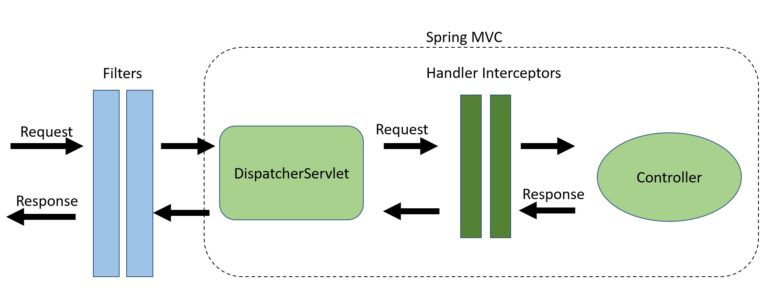
\includegraphics[scale=0.4]{filtervsinterceptor.png}
	\caption{Filter和Interceptor区别}
	\label{fig:filtervsinterceptor}
\end{figure}


https://segmentfault.com/a/1190000022833940

https://www.cnblogs.com/junzi2099/p/8022058.html

\end{document}





